\documentclass{article}
\usepackage[utf8x]{inputenc}

\usepackage{xcolor}
% \AddToHook{shipout/before}{%
%   \ifodd\value{page}
%     \pagecolor{blue!10!white}% Odd page colour (light blue)
%   \else
%     \pagecolor{red!10!white}% Even page colour (light red)
%   \fi
% }


\usepackage{geometry}
\geometry{letterpaper, margin=1in}

\providecommand{\tightlist}{%
  \setlength{\itemsep}{0pt}\setlength{\parskip}{0pt}}

\usepackage{adjustbox}
\usepackage[hyphens]{url}
\usepackage{lineno,hyperref}
\modulolinenumbers[5]

%% APA style
\usepackage{graphicx}
\usepackage{caption}

\definecolor{aqua}{rgb}{0.0, 1.0, 1.0}
\definecolor{deepmagenta}{rgb}{0.8, 0.0, 0.8}
\definecolor{almond}{rgb}{0.94, 0.87, 0.8}
\usepackage{pagecolor}
\usepackage{afterpage}

\begin{document}
\pagestyle{empty}
\thispagestyle{empty}
\pagecolor{aqua!30}

\begin{figure}[h]
\begin{adjustbox}{minipage=[c]{\textwidth-10mm},margin= 5mm 15mm 5mm 13mm, frame=1pt, bgcolor=almond,env=center}%
%\begin{adjustbox}{varwidth=\textwidth,bgcolor=almond,margin=3mm {\abovecaptionskip} 3mm 3mm, frame=1pt }
\begin{center}
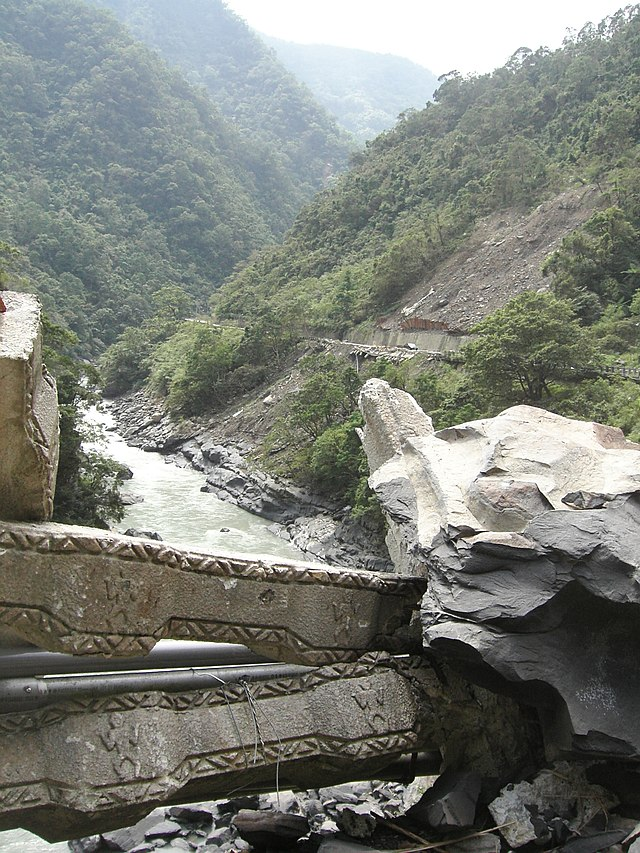
\includegraphics[trim=0mm 40mm 0mm 40mm, clip,width=.6\paperwidth]{river_damage.jpg}
\end{center}

\begin{center}
\begin{minipage}[t]{0.7\paperwidth}

\medskip
{\huge Historian}
\bigskip

\Large\raggedright
\textbf{Context} When developing a vision of the future.\newline
\textbf{If} people start to agree BUT no one connects it with local history and concrete actions, then work bogs down;\newline
\textbf{Then} use words like “\emph{specifically}” to connect abstract problems and solutions to specific actions.
\end{minipage}
\end{center}
\caption*{2005 October 12, river damage seen during hike south of Taipei  by user Syced. Public domain, via Wikimedia Commons.\newline
\url{https://commons.wikimedia.org/wiki/File:2005_October_12,_river_damage_seen_during_hike_south_of_Taipei_11.jpg}}
\end{adjustbox}
\end{figure}

\end{document}